\documentclass[12pt]{article}
\usepackage[utf8]{inputenc}
\usepackage{graphicx}
\graphicspath{ {./images/} }
\title{Auctioneer}
\author{Andrei Maga}
\date{Noiembrie 2021}

\begin{document}

	\begin{titlepage}
		
		\maketitle
	\end{titlepage}
	\pagebreak
	
	\section{Descriere}
	Aplicatia modeleaza un sistem de licitatii online, pornind de la fundamentele unei licitatii fizice si transpunandu-le in mediul virtual. Este dotata cu propriul sistem de Escrow, insemnand ca pana la sfarsitul licitatiei, sistemul detine ambele bunuri (atat produsul cat si forma de plata) urmand ca dupa finalizarea acesteia sa realizeze distribuirea lor catre partile corespunzatoare.
	
	Un client inregistrat pe platforma are posibilitatea sa participe la licitatii deschise de alti clienti sau, sub anumite conditii de validare, poate deschide el insusi o licitatie.\\
	Lista licitatiilor este afisata pe pagina principala a aplicatiei, fiind ordonata in functie de activitatea desfasurata in cadrul fiecareia dintre acestea.
	De asemenea, clientul poate sa aplice diferite filtre asupra acestora in functie de categoriile sale de interes.

	\pagebreak

	\section{Arhitectura}
	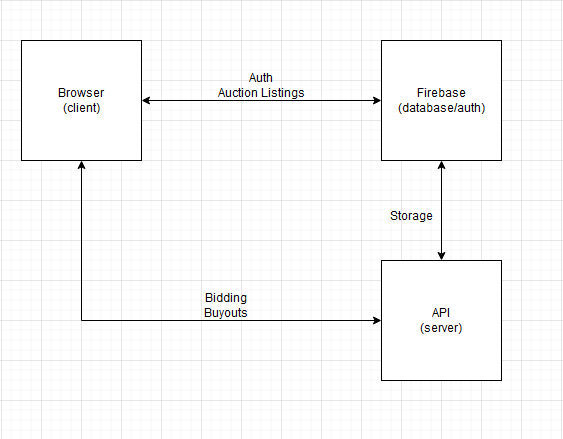
\includegraphics{archi}

\end{document}